\documentclass{article}\usepackage[]{graphicx}\usepackage[]{color}
% maxwidth is the original width if it is less than linewidth
% otherwise use linewidth (to make sure the graphics do not exceed the margin)
\makeatletter
\def\maxwidth{ %
  \ifdim\Gin@nat@width>\linewidth
    \linewidth
  \else
    \Gin@nat@width
  \fi
}
\makeatother

\definecolor{fgcolor}{rgb}{0.345, 0.345, 0.345}
\newcommand{\hlnum}[1]{\textcolor[rgb]{0.686,0.059,0.569}{#1}}%
\newcommand{\hlstr}[1]{\textcolor[rgb]{0.192,0.494,0.8}{#1}}%
\newcommand{\hlcom}[1]{\textcolor[rgb]{0.678,0.584,0.686}{\textit{#1}}}%
\newcommand{\hlopt}[1]{\textcolor[rgb]{0,0,0}{#1}}%
\newcommand{\hlstd}[1]{\textcolor[rgb]{0.345,0.345,0.345}{#1}}%
\newcommand{\hlkwa}[1]{\textcolor[rgb]{0.161,0.373,0.58}{\textbf{#1}}}%
\newcommand{\hlkwb}[1]{\textcolor[rgb]{0.69,0.353,0.396}{#1}}%
\newcommand{\hlkwc}[1]{\textcolor[rgb]{0.333,0.667,0.333}{#1}}%
\newcommand{\hlkwd}[1]{\textcolor[rgb]{0.737,0.353,0.396}{\textbf{#1}}}%
\let\hlipl\hlkwb

\usepackage{framed}
\makeatletter
\newenvironment{kframe}{%
 \def\at@end@of@kframe{}%
 \ifinner\ifhmode%
  \def\at@end@of@kframe{\end{minipage}}%
  \begin{minipage}{\columnwidth}%
 \fi\fi%
 \def\FrameCommand##1{\hskip\@totalleftmargin \hskip-\fboxsep
 \colorbox{shadecolor}{##1}\hskip-\fboxsep
     % There is no \\@totalrightmargin, so:
     \hskip-\linewidth \hskip-\@totalleftmargin \hskip\columnwidth}%
 \MakeFramed {\advance\hsize-\width
   \@totalleftmargin\z@ \linewidth\hsize
   \@setminipage}}%
 {\par\unskip\endMakeFramed%
 \at@end@of@kframe}
\makeatother

\definecolor{shadecolor}{rgb}{.97, .97, .97}
\definecolor{messagecolor}{rgb}{0, 0, 0}
\definecolor{warningcolor}{rgb}{1, 0, 1}
\definecolor{errorcolor}{rgb}{1, 0, 0}
\newenvironment{knitrout}{}{} % an empty environment to be redefined in TeX

\usepackage{alltt}
\usepackage{hyperref}

\hypersetup{
    colorlinks=true,
    linkcolor=blue,
    filecolor=magenta,      
    urlcolor=cyan,
}

\usepackage{listings}
\usepackage{color}

\definecolor{dkgreen}{rgb}{0,0.6,0}
\definecolor{gray}{rgb}{0.5,0.5,0.5}
\definecolor{mauve}{rgb}{0.58,0,0.82}

\lstset{frame=tb,
  language=bash,
  aboveskip=3mm,
  belowskip=3mm,
  showstringspaces=false,
  columns=flexible,
  basicstyle={\small\ttfamily},
  numbers=none,
  numberstyle=\tiny\color{gray},
  keywordstyle=\color{blue},
  commentstyle=\color{dkgreen},
  stringstyle=\color{mauve},
  breaklines=true,
  breakatwhitespace=true,
  tabsize=3
}


\author{Anna Burns \& Marc Los Huertos}
\title{Introduction to Raspberry Pi in Environmental Science}
\IfFileExists{upquote.sty}{\usepackage{upquote}}{}
\begin{document}
\maketitle

%\tableofcontents

\newpage

\section{Introduction}

\subsection{What is Rasberry Pi?}

The Raspberry Pi is an tiny computer, that includes a microprocessor, a bit of memory, a slot for an SD card, and some input/output jacks, e.g. HDMI, USB, headphone, camera, and pin headers for various sensors.

\subsection{Why use Raspberry Pi?}

The Pi has a lot of functionality and flexibility to develop monitoring of environmental parameters. 

\subsection{Uses in Environmental Science}

\subsubsection{Weather and Climate Change}

\subsubsection{Air Pollution Monitoring}

Raspberry Pi can also be used to monitor air quality. For a quick introduction, watch \href{https://use.vg/hDDhGdtnuhPT}{Marc's video describing the use of the Pi} to monitor air pollution. 

\subsubsection{Soil Water Monitoring and Irrigation Control}

The automatation of irrigation is ubiquitous, however, in many cases systems don't have feedbacks that control the system. The first step relies on sensors to monitor soil moisture and temperature and then uses plant growth models to control an irrigation system. 

Here are some resources that describe how these can be done:

\begin{itemize}
\item \href{https://fyi.extension.wisc.edu/cropirrigation/files/2015/03/Methods.to_.Monitor.Soil_.Moisture.pdf}{Soil Moisture Sensors and Loggers}
\end{itemize}

\subsubsection{Conservation} 

Conservation biologists use a wide range of instruments to track and monitor wildlife (camera traps, active (radio) and passive (RIF) transmitters). In addition the use of cameras are used to evaluate plant health and diversity (spectral analysis). 

\section{Resources}

\subsection{Resources}

\subsection{Raspberry Pi Foundation}

The Raspberry was created to help non-technical youth learn computing and robotics. The Raspberry Pi was an unexpected success and now the Pi is one of the most important minaturized computers for a wide range of projects.  

The \href{https://www.raspberrypi.org/}{RaspberryPi.org} has tutorials, software updates, and example projects.

\subsubsection{Video Tutorials}

One good way to start is to watch the following video series that introduced the Raspberry Pi. 

%\href{https://www.amazon.com/gp/video/detail/B07ZTR6ST2/ref=atv_dp_share_cu_r}{Amazon Prime -- Introducing Rasberry Pi History, Models, and Uses}

\subsection{Unpacking the Raspberry Pi}

We have three different models of Raspberry Pi, 3B version 2, 4B version X, and Zero W version X. The set up is slighly different for each. 

When you recieve your Pi, plan on spending about 1-2 hours setting it up which include unpacking and putting the Pi together: 

\begin{enumerate}

\item Unpack Kit Contents

\item Put Pi in case and add heat sinks if included or not previously installed

\end{enumerate}

\section{Setting Up Raspberry Pi}

In order to set up your Raspberry Pi, you will need one of two things: access to a USB-connected mouse and keyboard as well as a monitor that allows you to connect via HDMI (TVs or desktop computers both have this capability); or a computer that can read an SD card.  The first of these options is simplest; if you do not have access, use option two for the SD-card option.  If you do not have access to either, contact your professor so that they can get a monitor, keyboard, and mouse to you.

\subsection{Option 1: Direct Access with the Pi using a Monitor, Keyboard, and Mouse}

If you have a spare monitor, keyboard, and mouse, use the following steps to set up the Raspberry Pi. If you don't have these, but do have a slot on your computer for an SD card, then follow the instructions in Option 2.

\begin{enumerate}

\item Connect to keyboard, mouse and monitor. Make sure the HDMI plug is in the correct mini-HDMI socket and the monitor is configured to get a signal from the port being used. 

\item Insert pre-loaded SD card. If the SD care does not have the operating system (OS), then see the SOP for ``Imaging the Pi SD Card''. 

\item Plug-in Pi, you'll see a rainbow screen for a minute and then a installation menu. 

\item Install the Rasbian operating system only. This will take 10 minutes. Read the little windows so you know some of the resources associated with the operating system. The installations stalls at the end, where it says 100\%. Be patient, it will finish on it's own and reboot.

\item Once the Rasbian OS starts, you'll see four raspberries at the top and then you'd get some prompts to set up the OS. 

\item I suggest you keep the username and password as default for now, select the langauge, keyboard type, and time zone. 

\item Next you'll need to get connected to the internet. Select your modem and enter password to connect.

\item Then you'll get a prompt to check for updates. Yes, there will be updates. This will take another 20 minutes. About halfway the screen goes completely blank. This is because, by default, the Pi goes into screen saver mode without mouse or keyboard inputs. Move the mouse or type something and the screen should wake up. 

\item Be sure to shut down your Raspberry Pi before unplugging it; you can use the keyboard and "Ctrl-Alt-Delete" sequence to get a pop-up window to shut the Pi down or open the terminal window and type:

\begin{lstlisting}
$ sudo shutdown -h now
\end{lstlisting}

\item You have successfully communicated with the Pi!  

\item Unplug the Pi.

Note: To restart the Pi, simply plug it in, unless you have a switch.

You can access your Pi via a monitor; however, if you would access your Pi via a computer, follow the guide for "Option 3: Remote Access on a Configured Pi". 

\item Follow the instructions to update the Pi's OS (Section: \ref{subsec:OS}).

\end{enumerate}

\subsection{Option 2: Remote ssh Access}\label{subsec:Option2}

If you do not have access to a keyboard, mouse, and monitor, but do have access to a laptop with an SD card slot, this option is for you.  Once you go through these steps, you will be ready to begin working on your Pi remotely (and thus will not need to follow the instructions in the following section, ``Remote Access on a Configured Pi'').

We created pre-downloaded SD card with the various operating systems already downloaded; you need to select which one you would like (Raspain), and you then need to add files to the boot on the SD card so that your Pi can connect to Wifi and the SSH is enabled.  Finally, you need to find your Pi's specific IP address so that you can connect remotely, and then you can access your Pi via SSH!

Source: %\href{https://medium.com/@maheshsenni/setting-up-a-raspberry-pi-without-keyboard-and-mouse-headless-9359e0926807}{Setting Up Raspberry Pi Without a Keyboard or Mouse (Headless)}

\begin{enumerate}

\item Make sure that your Pi is NOT connected to a power source, and remove the MicroSD card.

\item Insert the MicroSD card into a computer; the process for this is different for each computer, and you can Google how to insert a MicroSD card for the model computer you are using.  It will look like a small slot (about 1 cm wide), and when you insert the card it should click in.

\item Open the sd card on your computer. 

\item Ensure you have the pre-configured boot SD card installed in the Pi with numerous files.

\item Create or open a document named ``wpa\_supplicant.conf'' as described below:

\begin{description}
  \item[Mac instructions] Create a new empty file that will hold network info:

\begin{lstlisting}
touch /Volumes/boot/wpa_supplicant.conf
\end{lstlisting}

\item[Windows instructions] Start Notepad. Paste in the contents below (adjusting for the name of your country code, network name and network password). Click File / Save As. Be sure to set Save as type to All Files (so the file is NOT saved with a .txt extension). Call the file ``wpa\_supplicant.conf'' and save it.  Close the file. If you see a .txt extension, you can also rename the file without the extension. 
\end{description}

\item Then paste the following into it (adjusting for your ISO 3166 alpha-2 country code, your wifi network name and network password):

\begin{lstlisting}
country=US
ctrl_interface=DIR=/var/run/wpa_supplicant GROUP=netdev
update_config=1

network={
    ssid="NETWORK-NAME"
    psk="NETWORK-PASSWORD"
}
\end{lstlisting}

Check that you have inserted three things: your 2 letter ISO country code (if you are in the United States, this is US); your Wifi's name; and Wifi's password.  Note be sure to include quotation marks around your ssid and psk (passkey).

\item Next, if there is no file called in the directory, create a file named ``ssh'' using one of the following methods:

\begin{description}
  \item[For Macs] we use the ``touch'' command to create the file.
  
\begin{lstlisting}
touch ssh
\end{lstlisting}

\item[For PCs] Create a new file in notpad and file/save as ssh as an empty file.  Save the file within the boot folder on the SD card.  Note that if you are on Windows, make sure that the file type is ``all files'' and not ``txt''.

\end{description}

\item Double check that both of the files you created are within the boot folder, and then left-click on the folder and select ``eject''.  
\item Remove the SD card from your computer, and reinsert it into the Pi and plug the power cable into the Pi.

\item Your Pi is now configured, and now we can access make sure the network can find your Pi.

\item Determine your router IP address. One way it to look up the properties of your network connection and at the bottom you'll find the network IP address (Figure~\ref{fig:RouterIPAddress}), write down the IPv4 address. 

\begin{figure}
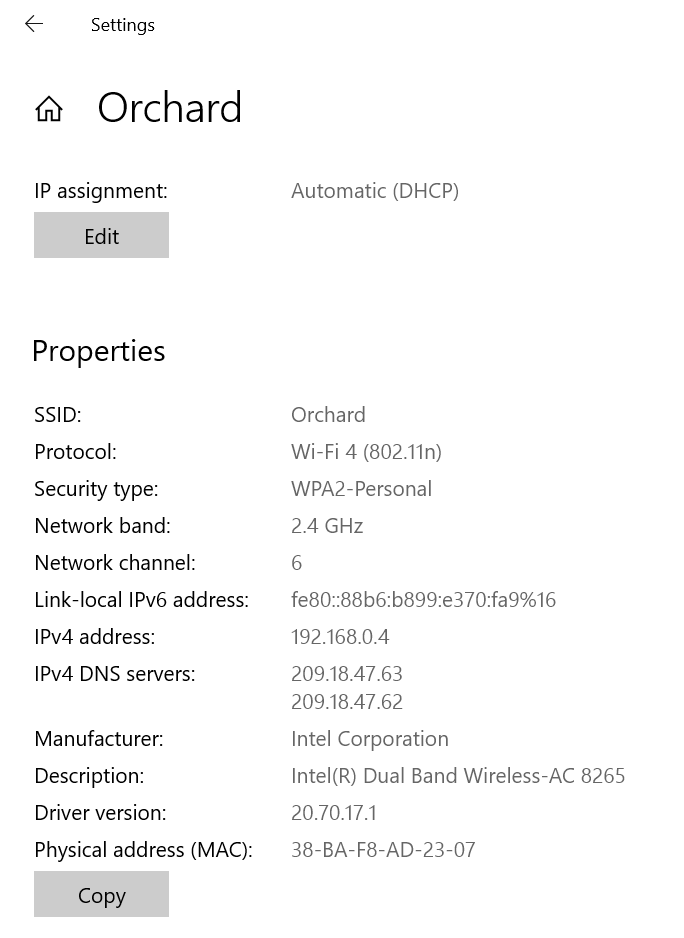
\includegraphics[width=\textwidth]{images/RouterIPAddress.png}
\caption{Determining the IP address of your router -- Note the 4 sets of numbers in the IPv4 Address, 192.168.0.4, this is an example of an router IP address.}
\label{fig:RouterIPAddress}
\end{figure}

\item Download \href{https://www.advanced-ip-scanner.com/}{``Advanced IP Scanner''} and scan using the IP address range of your router, e.g. 192.168.0.1-254, where we search between 192.168.0.1 and 192.168.0.254. FYI: What power of 2 is 254? Turns out it's 2$^8$ = 256, but two addresses are reserved. 255 on my network seems to be my computer and I don't get an entry for 0 and 256 is invalid. 

\begin{figure}
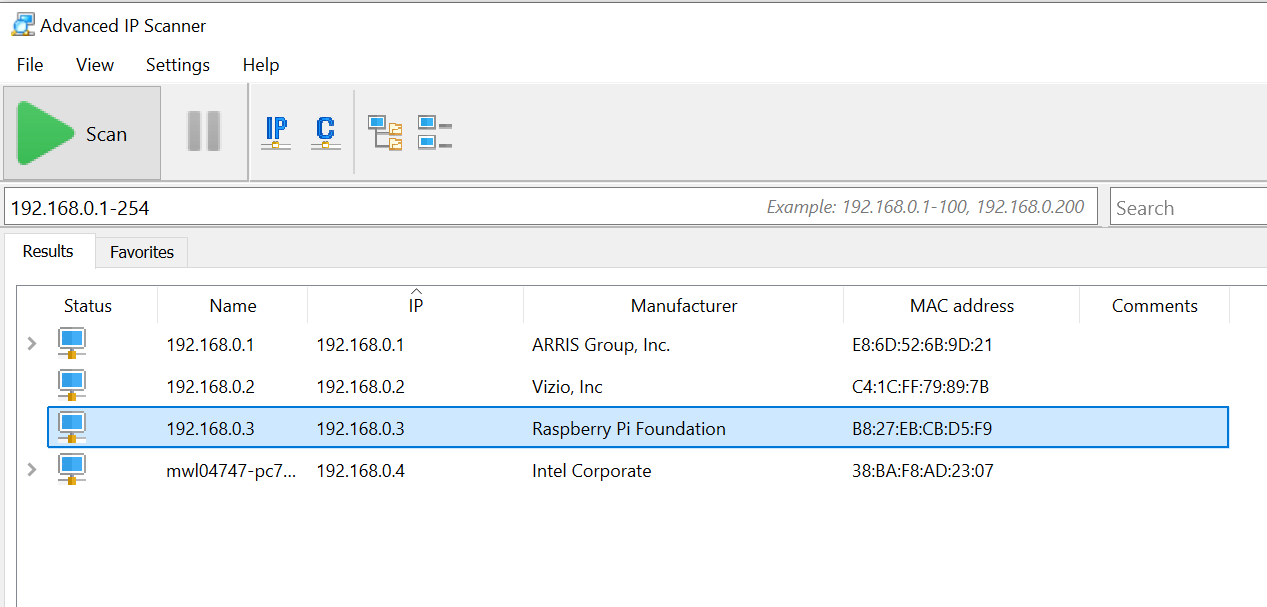
\includegraphics[width=\textwidth]{images/AdvancedIPScanner.png}
\caption{Determining the IP addresses used in your network.}
\label{fig:AdvancedIPAddress}
\end{figure}

Once this is complete, you will often see several devices in your network and hopefully you'll see the Raspberry Pi Foundation listed (Figure~\ref{fig:AdvancedIPAddress}). 
%it via SSH with the following instructions in your computer's shell.

\item Check to see if can communicate with the Pi. We use the ``ping'' command followed by the IP address. First, we need to open a ``command prompt'' window. 

\begin{lstlisting}
ping IPaddress
\end{lstlisting}

You should see some reference to the 4 packets sent and recieved and some reasonable amount of elapsed time (Figure~\ref{fig:Ping}). 

\begin{figure}
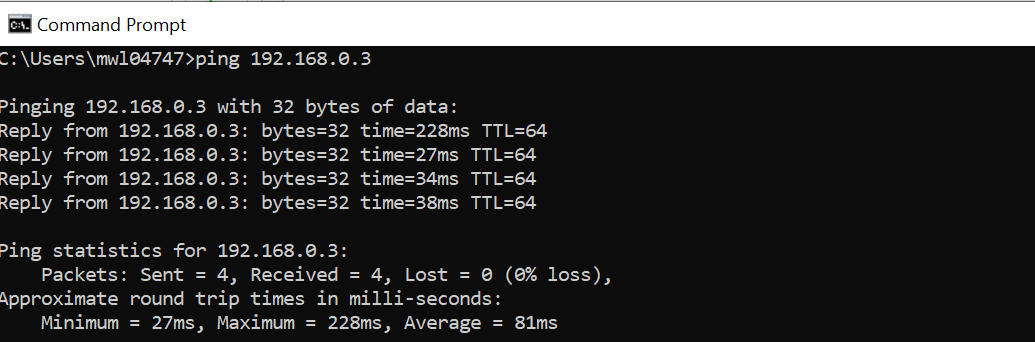
\includegraphics[width=\textwidth]{images/2-3_Ping_scn_shot.png}
\caption{Ensuring communication with Pi using ping}
\label{fig:Ping}
\end{figure}

\item Create an ssh connection. Uing the ``Command Prompt'', type 

\begin{lstlisting}
ssh username@IPaddress
\end{lstlisting}

Once you enter this command your computer  will ask if you trust it to create a paired communication key. Type ``yes'', and you shoul be set. 

\begin{figure}
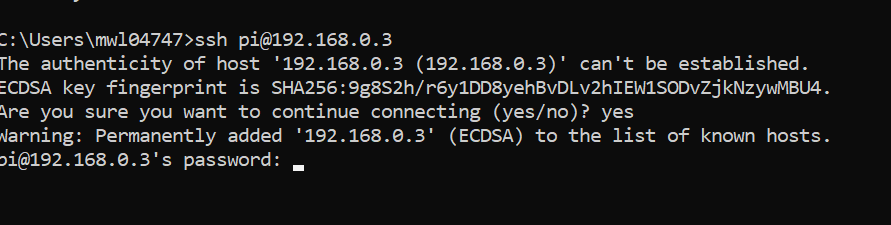
\includegraphics[width=\textwidth]{images/2-5_ssh_login_password.png}
\caption{Using ssh to login into the Pi for the first time will create a ssh key that allows your computer to be paired with the Pi.}
\label{fig:5_sshloginpass}
\end{figure}

However, there are times when you might get a conflict with the IP address assigned to a different device (Figure~\ref{fig:sshfail}).

\begin{figure}
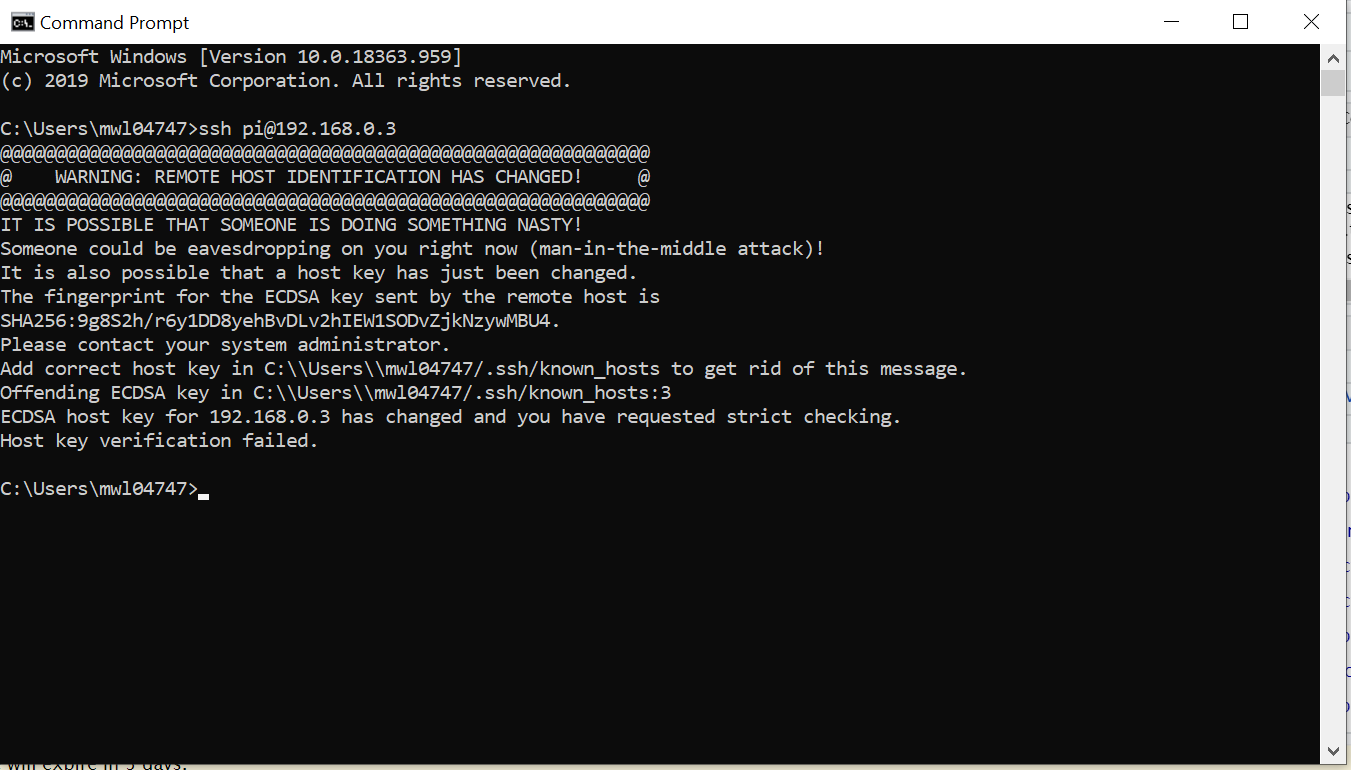
\includegraphics[width=\textwidth]{images/2-4_ssh_fail.png}
\caption{Host key verification failure means the IP address is assigned to a different paired device. You will need to find the file on your computer and edit out the conflicting device.}
\label{fig:sshfail}
\end{figure}

We suggest you get help if you are not able to figure this out. Save time to do other stuff!

\item Next the Pi will prompt you for the password. Note: As you type, no characters will appear on the terminal (for privacy).  This is ok, once you have typed your password just press enter.  If you didn't change your password during setup, it will be ``raspberry''.

\begin{figure}
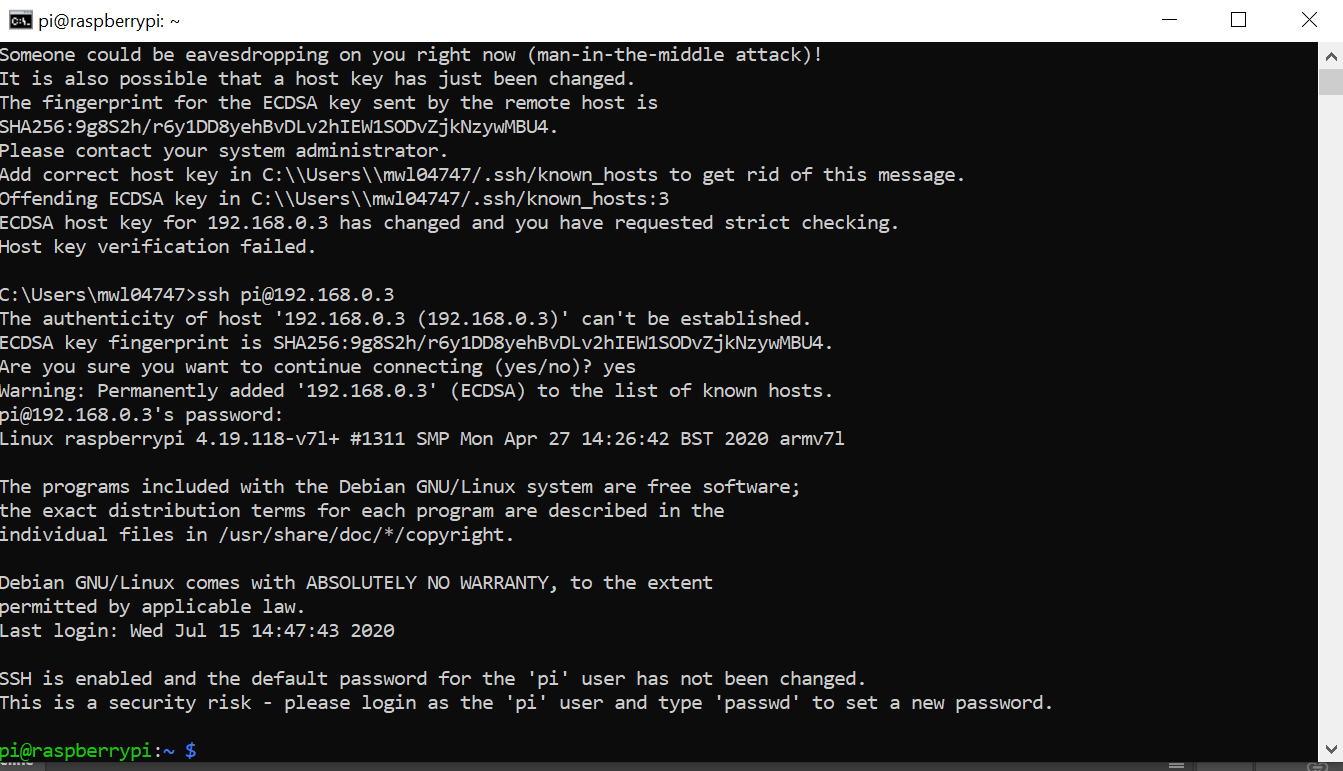
\includegraphics[width=\textwidth]{images/2-6_ssh_login_success.png}
\caption{A successful ssh connection should look something like this.}
\label{fig:6_sshsuccess}
\end{figure}

\item The terminal should now look like the Raspberry Pi terminal that you get via HDMI, with ``pi@raspberry pi: \$'' command prompt.  Hooray!

\begin{lstlisting}
ssh username@IPaddress
\end{lstlisting}

where the username is pi and the IP address you just found by pinging (it should look something like this: 192.168.X.X). If you changed your username during setup, then you'll type something other than ``pi''.

If you get some replys that look something like Figure~\ref{fig:1ping}, then the Pi is communicating accross the network. You have made progress!  If not, send a slack note to get help. 

\begin{figure}
\caption{Communicating with the Pi with ping. This screenshot is from the Windows command prompt.}
\label{fig:1ping}
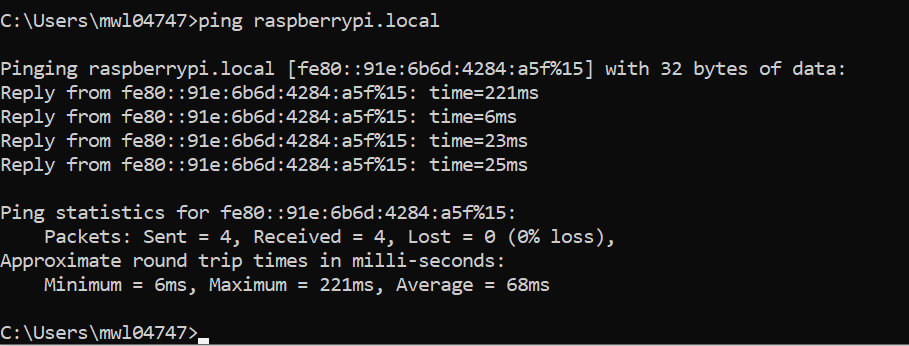
\includegraphics[width=\textwidth]{images/2-1_Ping_scn_shot.png}
\end{figure}

\item 

\end{enumerate}

\subsection{Option 3: Remote Access on a Configured Pi}

This section is for if you have already set up your Pi via a monitor, and would like to be able to access it via a laptop.  If you have not yet configured your Raspberry Pi with the correct operating systems and settings, please refer to the previous section, ``Remote Access Startup with the Pi.''

It doesn't take too long (10 minutes once you get the hang of it) to be able to work remotely on your microprocessor via a tablet or laptop.  
At first this requires being tethered to the use of a keyboard, mouse, and monitor, then you'll be free!

More information by reading \href{https://pythonprogramming.net/remote-access-raspberry-pi-tutorials/?completed=/introduction-raspberry-pi-tutorials/}{Remote Access with Raspberry Pi Tutorial} or \href{https://www.raspberrypi.org/documentation/remote-access/ip-address.md}{Remote Access Documentation}.

\begin{enumerate}

\item Begin by making sure all of your packages are up-to-date (even if you updated while setting up your OS, you will still need to do this).  Do this with the code 

\begin{lstlisting}
sudo apt-get update
\end{lstlisting}

and then 

\begin{lstlisting}
sudo apt-get upgrade
\end{lstlisting}

If there is an update, you will be asked to confirm the upgrade because it might take additional disk space. I don't see anyway around this, so type in Y. The update will will take several minutes. 

It might ask you to reboot, if so go for it and restart the terminal window. Either way, continue below.

\item Enable the SSH server by typing 

\begin{lstlisting}
sudo raspi-config
\end{lstlisting}

into the console.  This will lead you to a screen with several options; select option five, ``interfacing options,'' and then select option two for ``SSH.''  Enable the server, and then exit this screen.

\item Note that Raspberry Pi updated in November 2016 so that SSH is disabled automatically.  You will need to turn it on in order to progress.

\item You will need to know your Raspberry Pi's IP address \hypertarget{Pi's IP address} to connect to it. To find this, type 

\begin{lstlisting}
hostname -I 
\end{lstlisting}

from your Raspberry Pi terminal to find your Pi's IP address. This should be a string of numbers that looks something like ``192.168.XXX.XXX''.  You will need this to access your Raspberry Pi remotely. Find some paper and write down the number. 

\end{enumerate}

Before you proceed, look at the descriptions for options 3A and 3B below to see which is the right choice for your remote access needs.

\subsubsection{Option 3A: Remote Access to the Raspberry Pi GUI}

If you don't have much computer programming experience, this option may be better for you.  It allows you to access the actual Pi terminal (like the one you see when you connect an HTML cable) on another computer.  It is a more visually-friendly option, and allows you to directly access different apps through the Pi itself.

\begin{enumerate}

\item Install the package necessary to remotely access your screen: 

\begin{lstlisting}
sudo apt-get install xrdp
\end{lstlisting}

\item Connecting to Mac or Linux OS: open the terminal and type

\begin{lstlisting}
ssh pi@IPaddress
\end{lstlisting}

\item Connecting to Windows OS: this is a bit more involved; you might need to download an SSH client. 

\item The Microsoft ``Remote Desktop Connection'' app is available for free, and is pretty intuitive to use. Usually, this is already installed on the computer and you can find it by searching for the name using the tool bar search icon. If not, you may need to download the application, and follow the instructions to set it up. `Unfortunately, the ``Home'' version of MS Windows does NOT support RDC, so I suggest you look at these options: \url{https://www.itechtics.com/remote-desktop-windows-10-home/#Chrome_Remote_Desktop}. Instead it might be best to enable VNC and then use a VNC viewer. More soon!

\item Start the program and it will prompt you to enter the Pi's IP  address you found above into the text box (it should look something like 192.168.X.X).

\begin{figure}
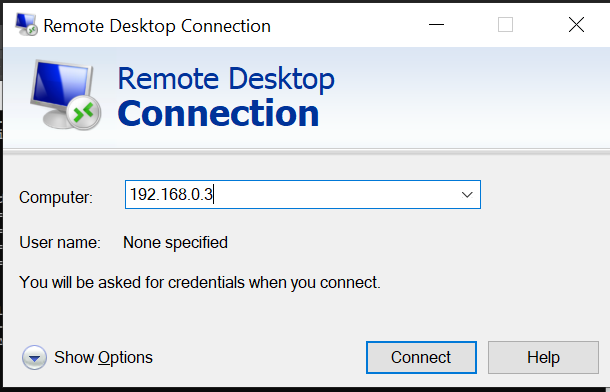
\includegraphics[width=\textwidth]{images/3A-1_Remote_Connection.png}
\caption{TBD}
\label{fig:3A-1}
\end{figure}

\item A page will open for you to add your username and password (which at this point should still be Pi's username and password, that is, ``pi'' and ``raspberry'').  Then your console will open.

\begin{figure}
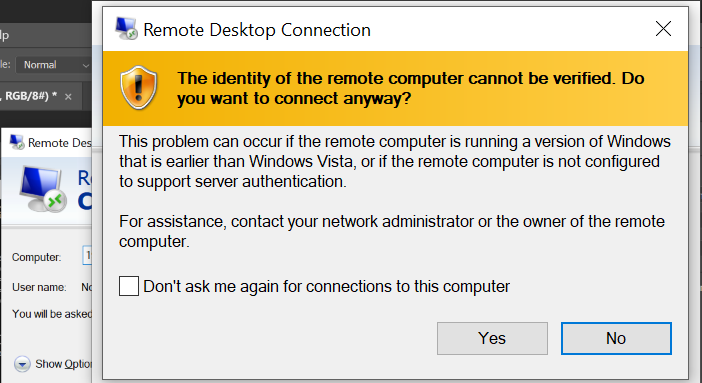
\includegraphics[width=\textwidth]{images/3A-2_Remote_Connection_Warning.png}
\caption{TBD}
\label{fig:3A-2}
\end{figure}

\item If it won't conect: make sure your microprocessor and the computer you are attempting to accesss it from are on the same wifi, you can check by using the \hyperlink{ping}{ping} command in the command window to confirm communications.

\item Make sure your microprocessor is connected and hasn't gone to sleep;

\item Make sure you've properly enabled all of the packages. Note: You may need to run the  xrdp twice to get it to work for the first time). 

\begin{figure}
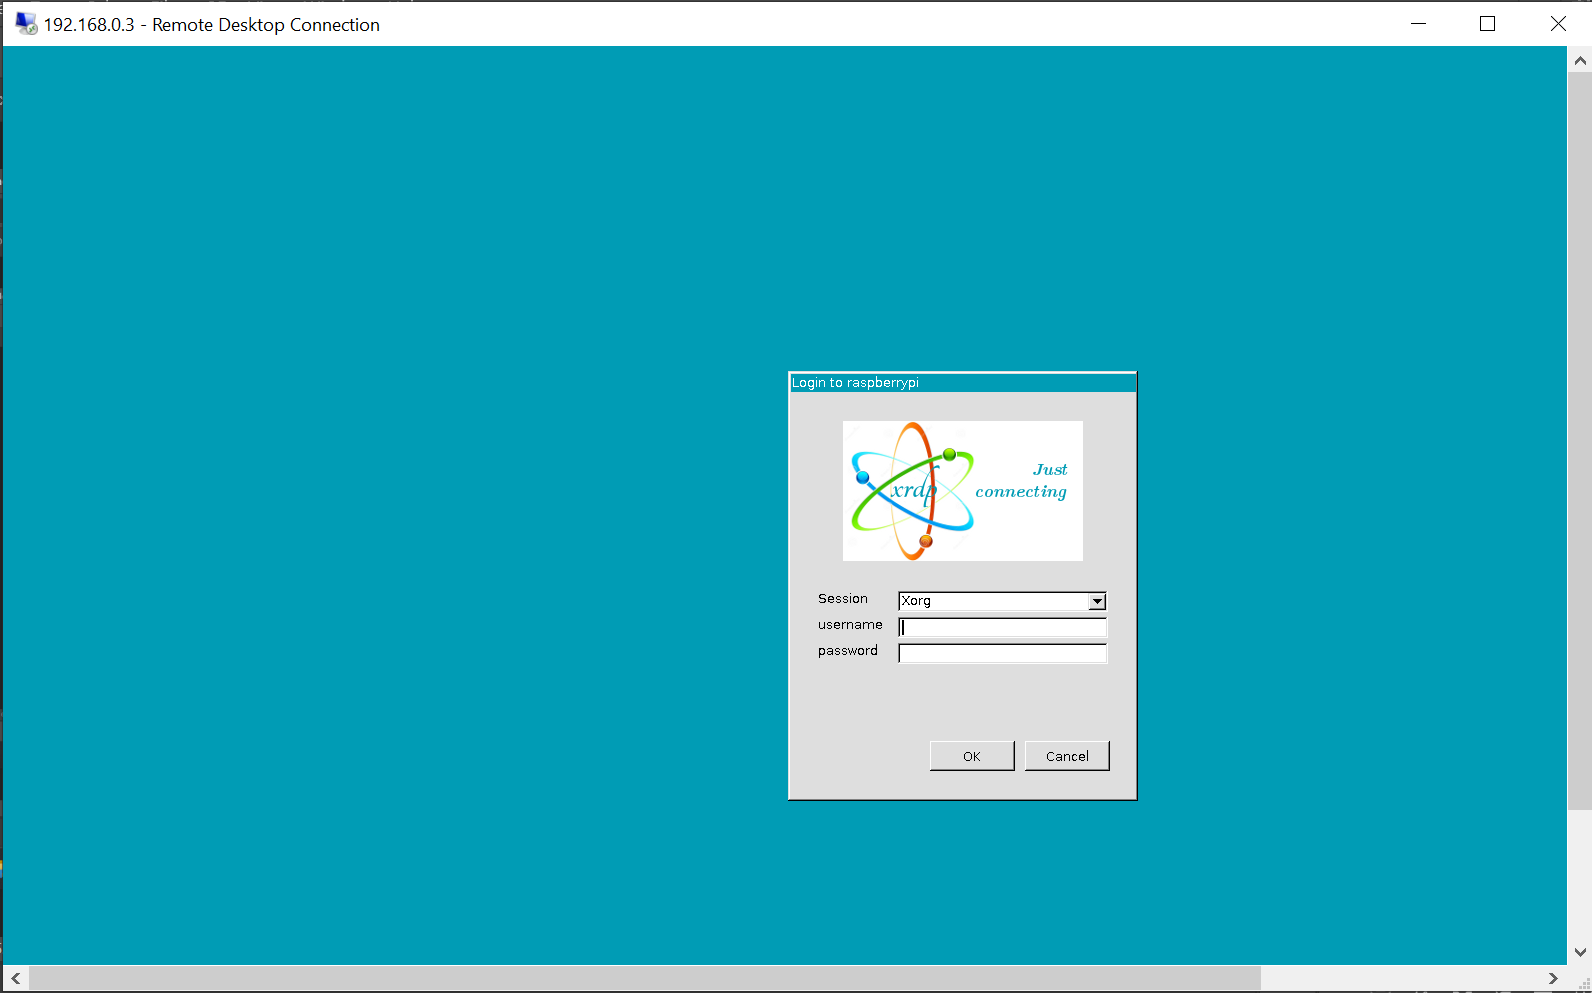
\includegraphics[width=\textwidth]{images/3A-3_Remote_Login.png}
\caption{TBD}
\label{fig:3A-3}
\end{figure}

\begin{figure}
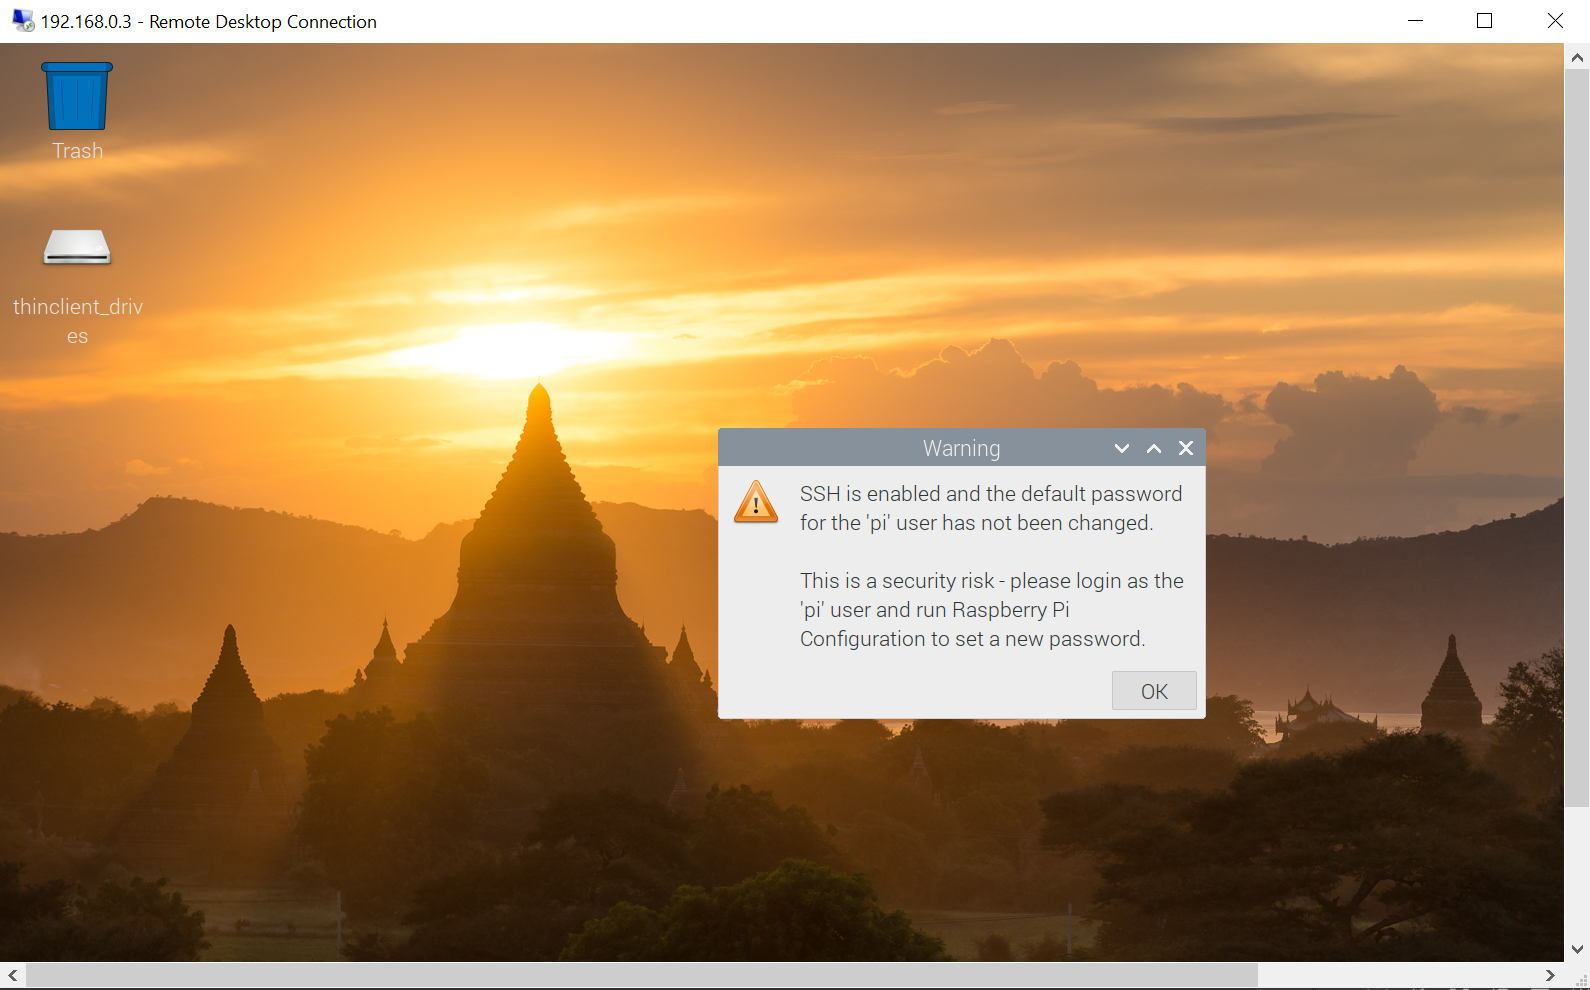
\includegraphics[width=\textwidth]{images/3A-4_Remote_Connected.png}
\caption{TBD}
\label{fig:3A-4}
\end{figure}

\item Now follow the instructions to update the Pi's OS (Section: \ref{subsec:OS}).

\end{enumerate}

\subsubsection{Option 3B: Remote Access to Raspberry Pi via SSH}

This option allows you to access your Pi microprocessor through an external shell, ``piggybacking'' the Pi onto an already existing computer.  It allows you to operate in raw code through an external frame, but does not have the visual appeal that the GUI does.  If you are more comfortable with programming, or feel familiar enough with navigating the Pi, this is the right option for you.

\begin{enumerate}

\item For Windows Only: (if you have Mac OS or Linux, skip this step!) Make sure you have OpenSSH Client installed. 

\begin{enumerate}

\item Open Windows Settings. If you are using Windows 10, click the Windows menu, and select the gear icon for Settings. 

\item Go to settings, Apps, ``Apps and Features'', Optional Features.

\item Click on Add a Feature.

\item Scroll down and add Open SSH Server.

\item Close the Settings Windows.

\end{enumerate}

%\item Ethernet IP Address: 192.168.137.1 

\item Open the Command Prompt (which is command line window in windows)

\item I recommend that you ``\hypertarget{ping}'' the Pi before going to the next step. Ping is a short command use to check of the communications are working. As it turns out if I am using Pomona's VPN, I could not get it to work. So, I disconnected from the VPN and then typed

\begin{lstlisting}
ping 192.168.0.4
\end{lstlisting}

If you get a series of packets and not a timeout error you are talking to your Pi! If not, stop -- don't get frustrated and contact your contact person for help!

\item Type

\begin{lstlisting}
ssh username@IPaddress
\end{lstlisting}

where the username is pi and the IP address is the number you wrote down in step 4 in section 2.2 (itshould look something like this: 192.168.X.X). If you changed your username during setup, then you'll type something other than ``pi''.

\item Once you press enter, it will ask if you trust it (say yes, you will only need to do this once). 

\item Next it will ask you for your password.  Note: As you type, no characters will appear on the terminal (for privacy).  This is ok, once you have typed your password just press enter.  If you didn't change your password during setup, it will be ``raspberry''.

\item The terminal should now look like the Raspberry Pi terminal that you get via HDMI, with ``pi@raspberry pi: \$'' command prompt.  Hooray! 

\item Now follow the instructions to update the Pi's OS (Section: \ref{subsec:OS}).

\item For further guidance, see the troubleshooting section.

\end{enumerate}

\subsection{Updating the OS}\label{subsec:OS}

\begin{enumerate}

\item Finally, you need to make sure your Pi is up to date.  Do this with the following lines within the Pi shell:
\begin{lstlisting}
sudo apt-get upgrade
sudo apt-get update
\end{lstlisting}
Since this is your first time using your Pi, this process could take several minutes.

\item Now that your Pi is updated, you can follow the instructions undersection 3A of ``Remote Access on a Configured Pi'' to access your Pi's GUI (user interface).  Instead of typing the commands into the Pi terminal in your monitor , you will do so in your computer's shell with the Pi shell piggybacked onto it.  Note that this guide takes you through a remote setup of option 2B of ``Remote Access on a Configured Pi'', and you will be able to follow the rest of the setup protocol without switching to a GUI.  Read the following section to see which option is right for you.

\end{enumerate}

\section{Troubleshooting}

\subsection{Unable establish ssh connection}

If you can ping, but the ``connection refused'', then the pi might not have the ssh enabled. 

If you are using a headless connection, see Section \ref{subsec:Option2} to make sure ssh has been enabled. Note: the file disappears after the Pi boots up, which usually means you have successfully enabebled the ssh.

If it is enabled, double check IP address on your router and the Pi's wpa\_

\subsection{Remote Access}

\begin{enumerate}

\item Your microprocessor needs to be connected to a powersource in order to remotely access it.

\item Both the GUI and main terminal options can be rather glitchy; if the program quits, wait a moment and then log back in.  It may not work on the first try, but do it again and it should connect.

\item Make sure that your computer is connected to Wifi, and that it is connected to the same Wifi network your microprocessor is on.

\end{enumerate}

\subsection{Headless SSH Connection}

If you need to connect your Pi microprocessor to a new Wifi network but do not have access to a monitor, follow this process. 

\begin{enumerate}



\item Using notepad, create a document named ``wpa\_supplicant.conf''. 

\item Insert the following code into the notepad document:

\begin{lstlisting}
ctrl_interface=DIR=/var/run/wpa_supplicant GROUP=netdev

update_config=1

country=Insert 2 letter ISO 3166-1 country code here

network={
 ssid="Name of your wireless LAN"
 psk="Password for your wireless LAN"
}
\end{lstlisting}

Being sure to insert three things: your 2 letter ISO country code (if you are in the United States, this is US); your Wifi's name; and your Wifi's password.  Note that there are meant to be quotation marks around your ssid and psk.

\item Within the notepad document, go into file/save as.  Save the file within the boot folder for the SD card.  Note that if you are on Windows, make sure that the file type is ``all files'' and not ``txt''.

\item Within your file directory, left-click on the ``boot'' folder and select eject.  You can now take out the SD card by pushing the card further in so that it un-clicks.

\item Reinsert the MicroSD card into the Pi, and continue the remote access connection in one of the methods discussed previously.

\item Note that even if you had already enabled SSH and found your pi's IP address on a previous network, connecting to a new network means that you need to re-establish SSH connections, AND that your Pi's IP address will (strangely) be different!  The remote connection will NOT work with the IP address you had used on your previous network connection.

\item To find your Pi's new IP address, connect the Pi to power and then enter the shell of a computer that is on the same wifi network as the Pi.  In the command line, ping your Pi by typing ``ping raspberrypi.local''.  This should give you the Pi's IP address, which should look something like ``192.168.X.XXX''.  You can use this to connect to your Pi via SSH with the instructions in ``Remote Access to a Configured Pi''.

\end{enumerate}

\section{Copying Files (e.g. python) on the Pi}

\subsection{USB}

\subsection{SD card}

\subsection{via Internet}

\subsubsection{curl}

curl is a command line program that can be used to get files from websites and install them directly onto your pi.



\begin{lstlisting}
curl -sSL URL | bash
\end{lstlisting}

When you use this command, you will get a warning, that downloading filed from the internet is inherantly unsafe, unless you trust the source with your virtual life. 

with the following arguments: 

\begin{itemize}
  \item -s silent mode
  \item -S show error (even when in silent mode)
  \item -L location, follow redirects (not sure what this means!
\end{itemize}



\subsubsection{github}


\section{Maintaining the Pi}

\subsection{Monitor the Pi's Temperature}

Right click on tool bar and ``Add/Remove Panel Items''. Then make sure the Panel Applets tab is selected, then click on the ``Add'' button. 
Add the ``CPU Temerature Monitor'' and close.

Follow the same steps to add the ``CPU usage monitor''.

\subsection{Screensaver}

The screen goes black after 10 minutes of inaction. This is a bit annoying since we are often doing things that take some time to sort out, i.e. more than 10 minutes. 

To turn this off you can a terminal window that allows you to type commands following the \$ prompt. 

Type the following command to turn off the screen saver using the following steps: 

\begin{enumerate}

\item Type: 

\begin{lstlisting}
sudo apt-get install xscreensaver
\end{lstlisting}

\item If this doesn't work, make sure your sudo is up to date with 
\begin{lstlisting}
sudo apt-get update
\end{lstlisting}

\item Once you've done this, go to the Raspberry icon in the upper-left corner and select ``preferences'' from the drop down menu.  Under ``preferences'' there is an option for ``screensaver''.

\item Once in screensaver, under the ``Mode'' dropdown you can select ``disable screensaver''.

\item Now your screen should stay awake even if you aren't actively using it.

\item More information/different methods are available at: \href{https://www.raspberrypi.org/forums/viewtopic.php?f=91&t=57552}{Pi Forum:  Disable Screensaver in Raspbian}

\end{enumerate}



\subsubsection{MOVE THIS to GIT SOP? Recovering Commits from Github}


If there is a conflict between commits and some information that was previously added to a file on R is lost, follow these steps to recover the information within previous commits.

\begin{enumerate}

\item Go to the project's Github page over the internet and open the page for the document you wish to recover code from.

\item On the bar before the file itself begins, select ``history'' on the right side of the screen.

\item Within the history tab, there should be a list of previous commits; select a commit that will have the code you are hoping to recover within it (i.e. if you were working on the code the previous Friday, select a commit from that day).

\item On the appropriate commit, select the ``<>" option on the right of the screen to open up a historic version of the repository from that day.  Note that this will direct you to the full repository from the time of the commit you select, and not just the document you are hoping to recover.

\item Go back to the document you need to recover code from, and open it.  It will have the historic code that was there at the time of the commit you selected; if you chose correctly, it should have the code you were looking to recover.

\item Copy the deleted lines of code out of the historic file, and into the document on R. 

\item Save the R document, commit, and push the information.  

\item The Github will remain on the historic commit until you leave the project; exit the entire project (for example, by going to the home screen on Github) and then re-enter the project to enter the up-to-date portal.

\end{enumerate}


\section{Implementing Pi Projects}

\subsection{Using Sensors with Pi}

Now the Pi is set up we can move on to developing environmental monitoring projects. 
\subsection{Using a Camera with Pi}


\end{document}
